Aqui ser� o espa�o para os anexos.

\section{Texto Base}

Artigo {\aspas{Part�culas e Intera��es} - Marco Ant�nio Moreira}.

\begin{figure}[ht]
	\centering
	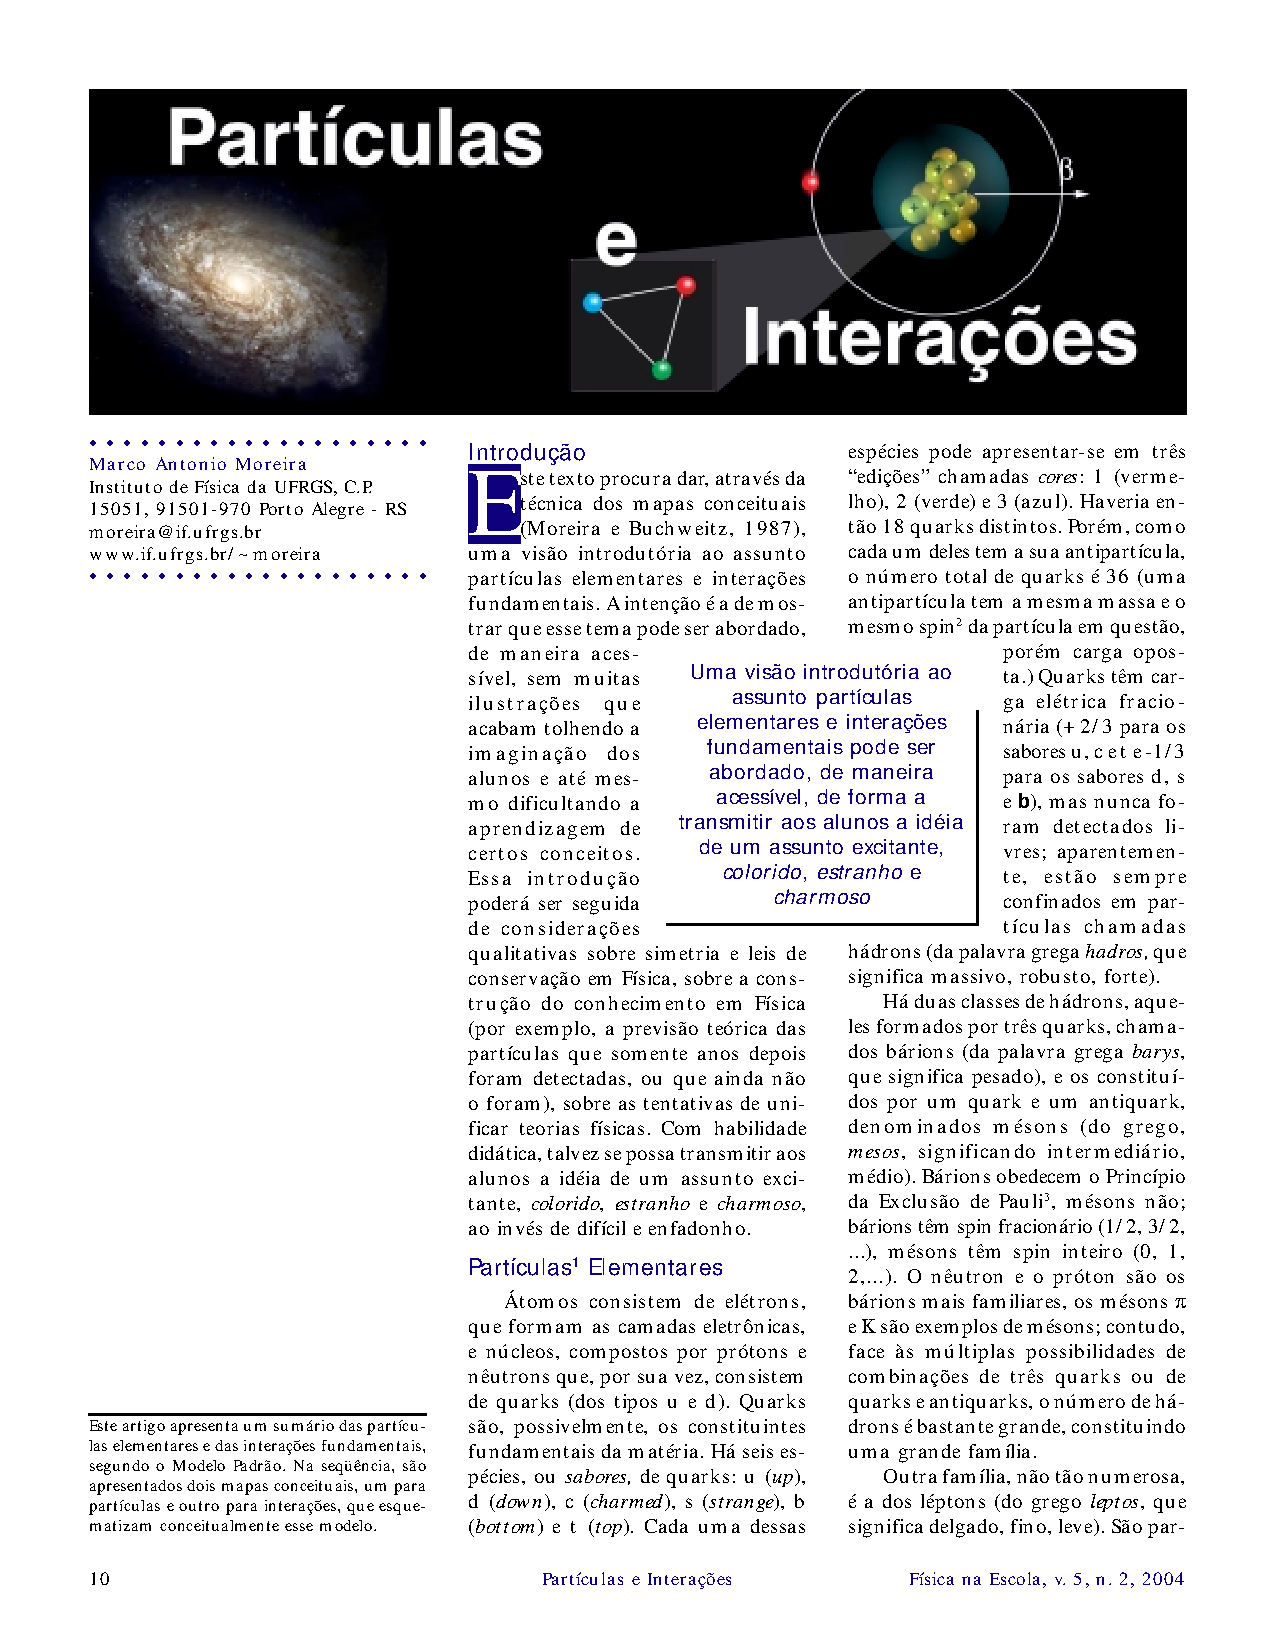
\includegraphics[width=1.0 \textwidth]{AneB/artigo_parte_1}
	\caption{Artigo: Part�culas e Intera��es - P�gina 1}
	\label{fig:artigo_parte_1}
\end{figure}

\begin{figure}[ht]
	\centering
	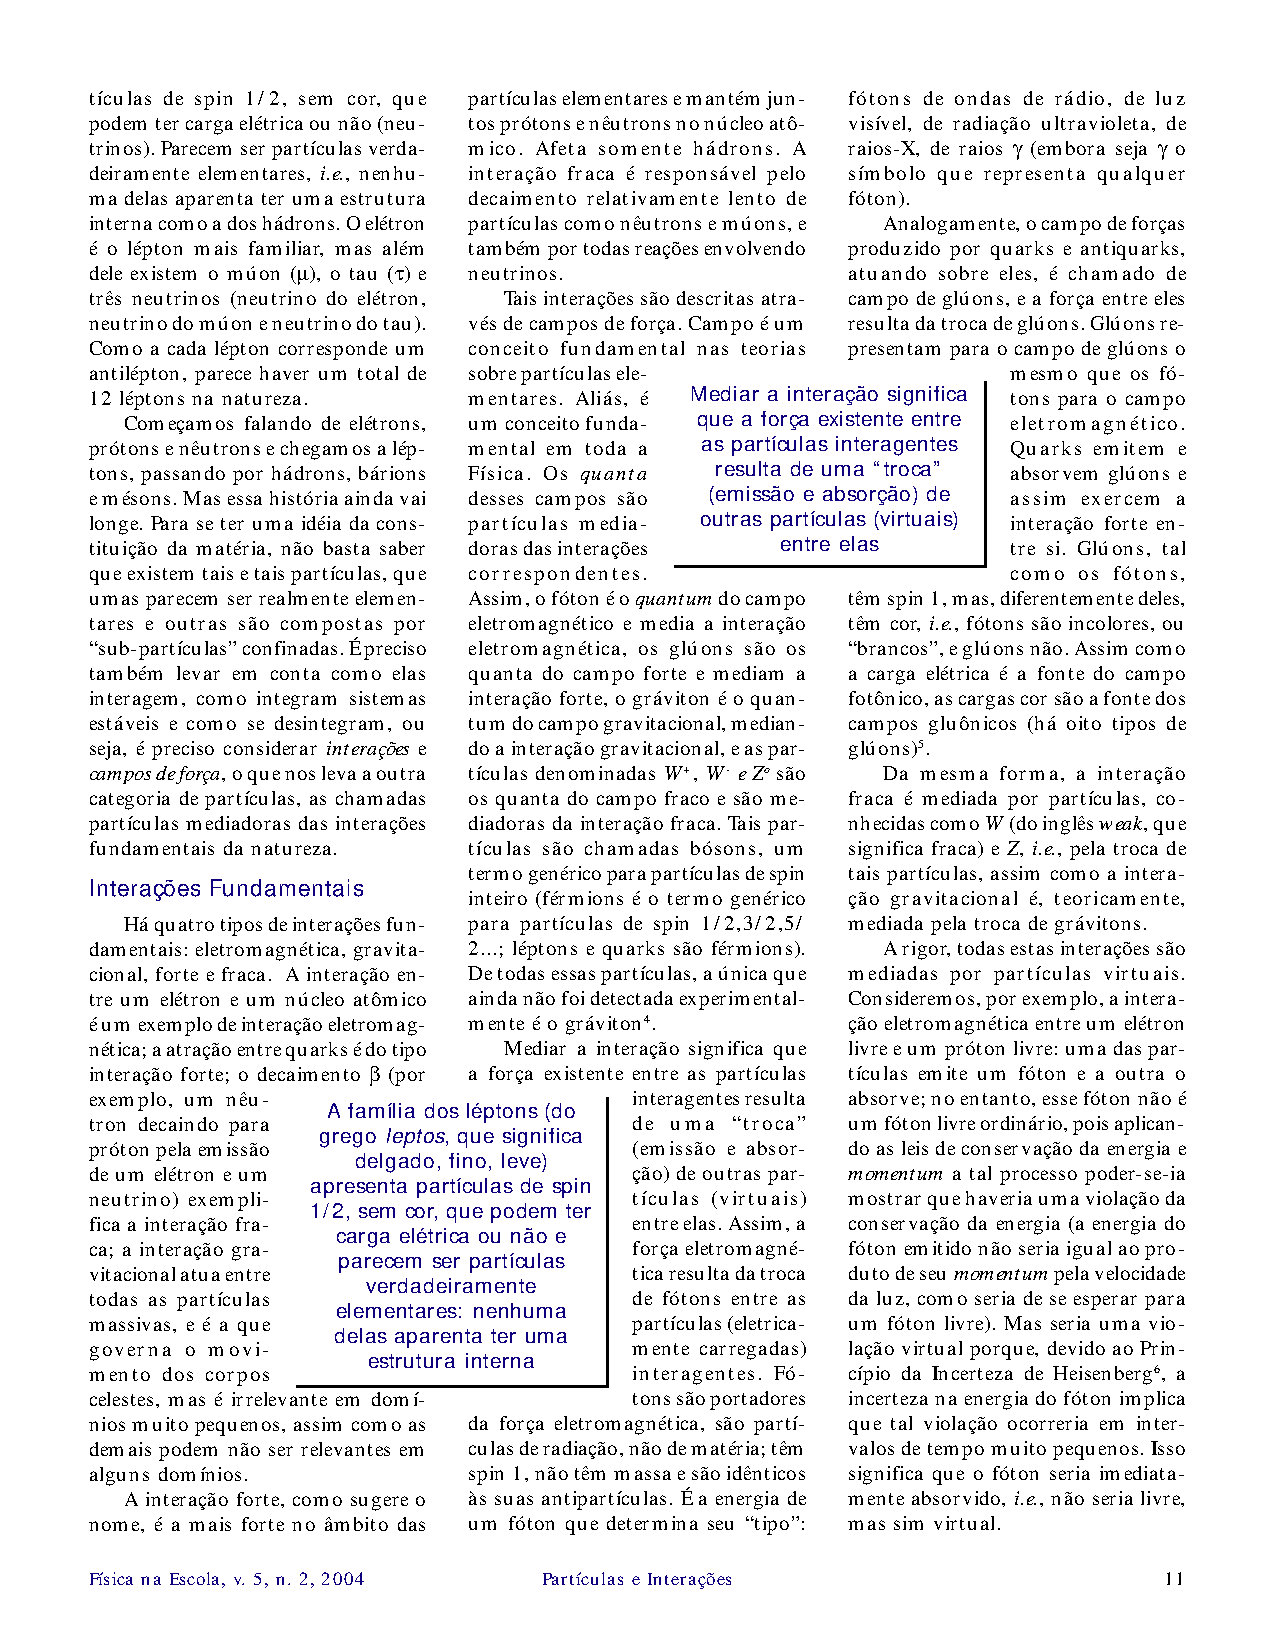
\includegraphics[width=1.0 \textwidth]{AneB/artigo_parte_2}
	\caption{Artigo: Part�culas e Intera��es - P�gina 2}
	\label{fig:artigo_parte_2}
\end{figure}

\begin{figure}[ht]
	\centering
	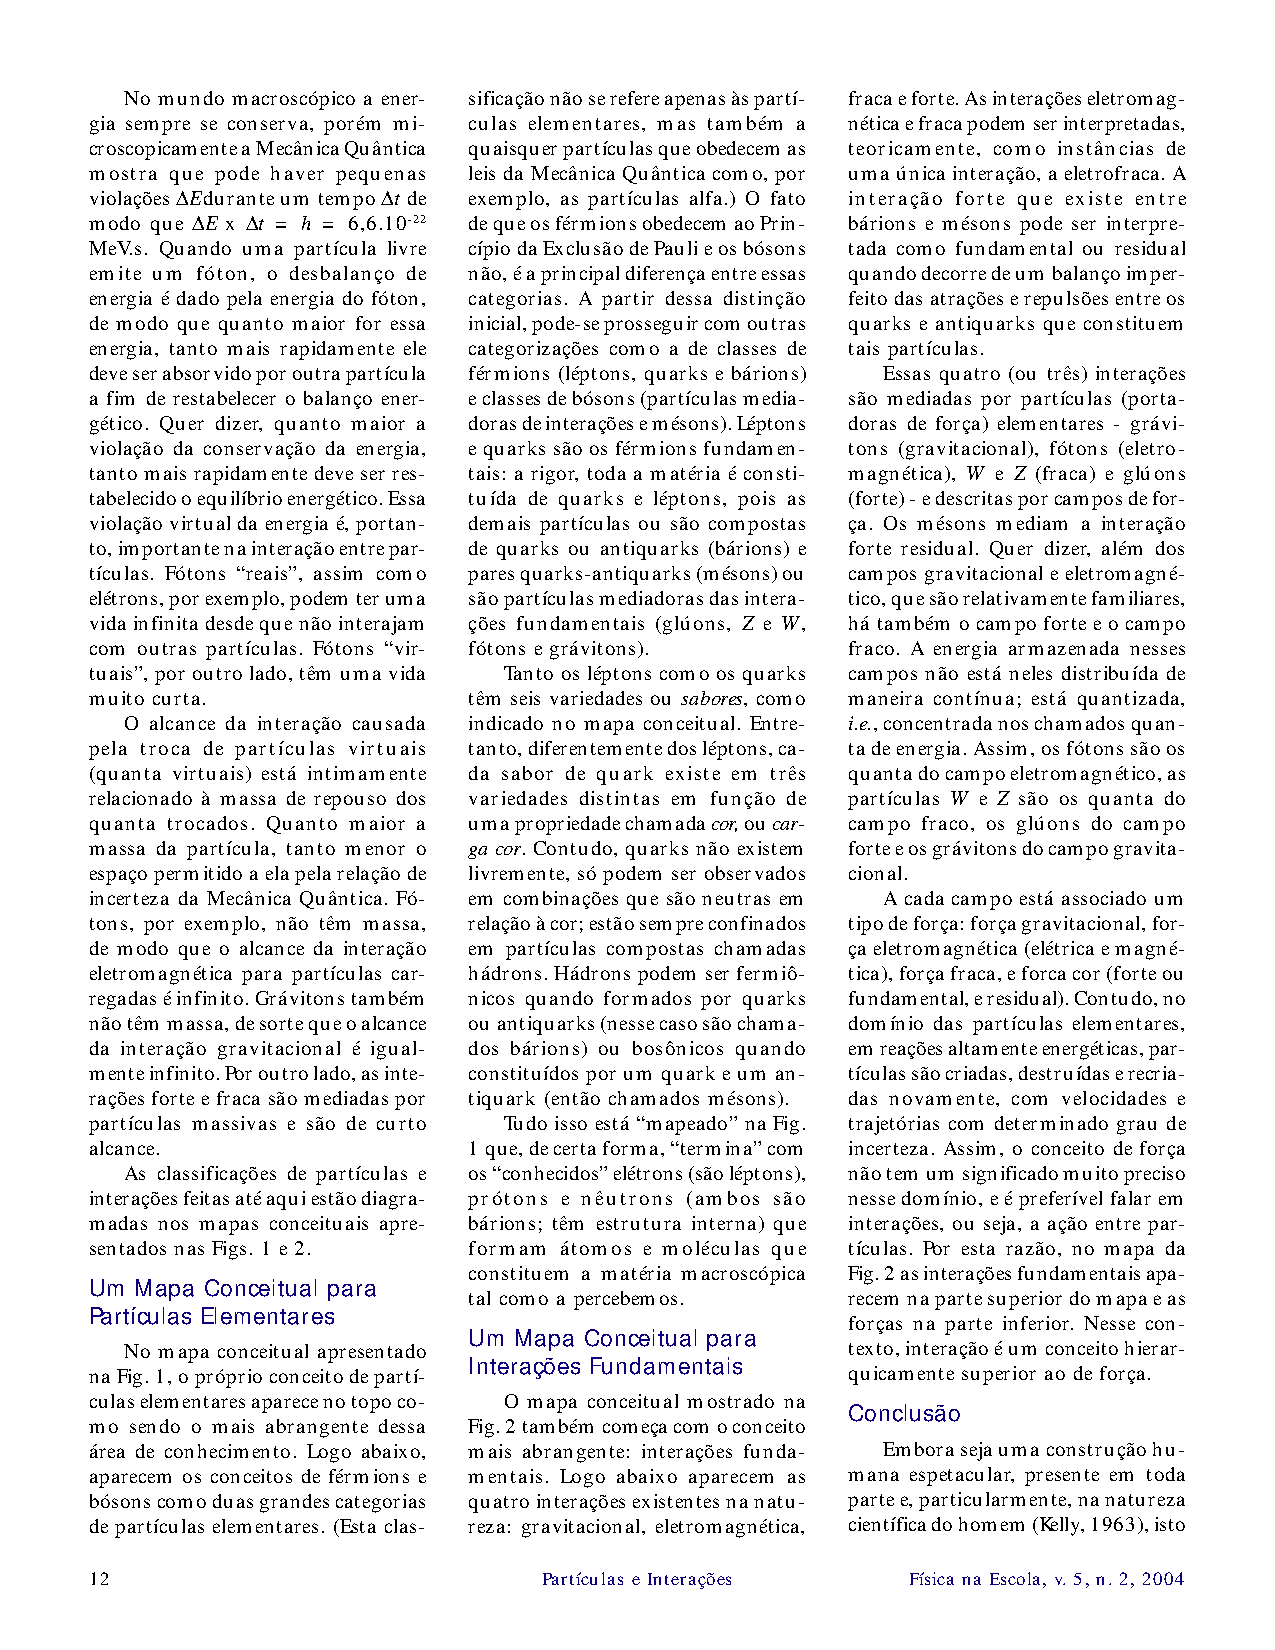
\includegraphics[width=1.0 \textwidth]{AneB/artigo_parte_3}
	\caption{Artigo: Part�culas e Intera��es - P�gina 3}
	\label{fig:artigo_parte_3}
\end{figure}

\begin{figure}[ht]
	\centering
	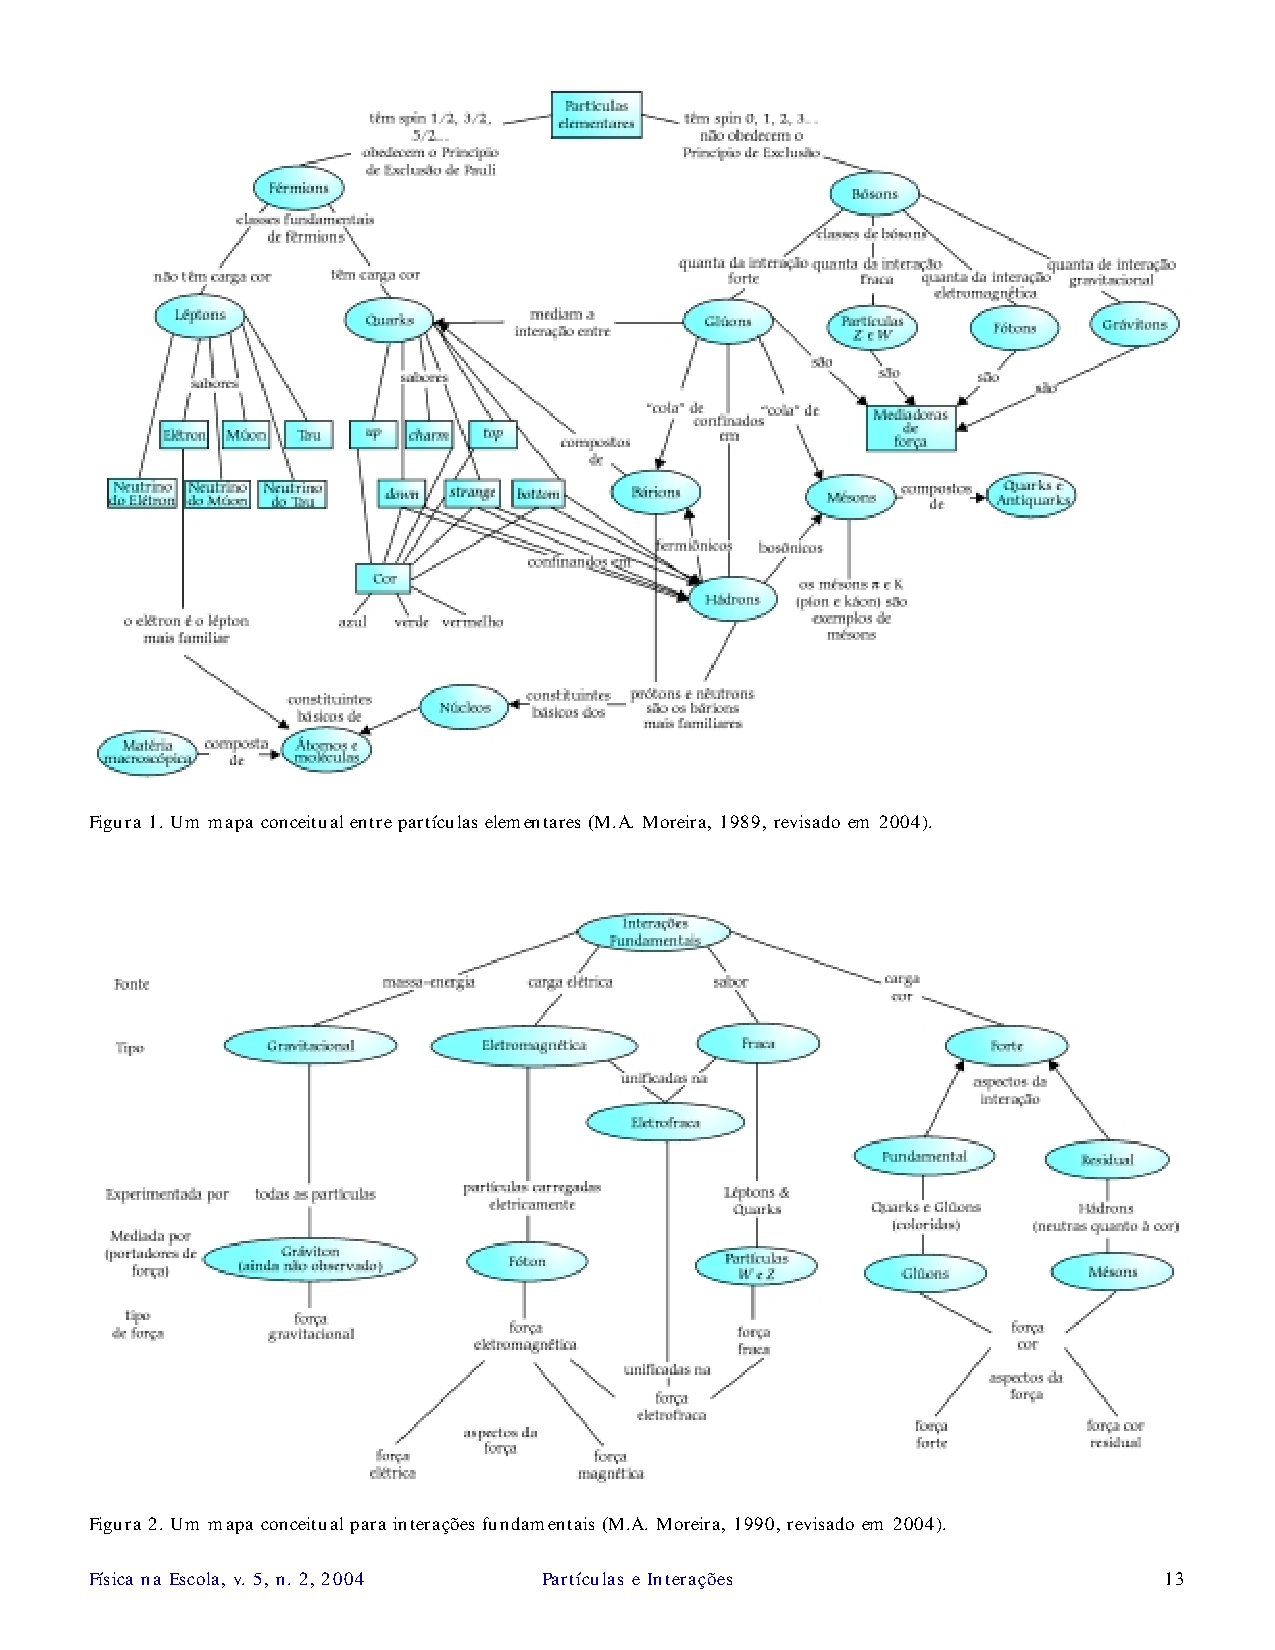
\includegraphics[width=1.0 \textwidth]{AneB/artigo_parte_4}
	\caption{Artigo: Part�culas e Intera��es - P�gina 4}
	\label{fig:artigo_parte_4}
\end{figure}

\begin{figure}[ht]
	\centering
	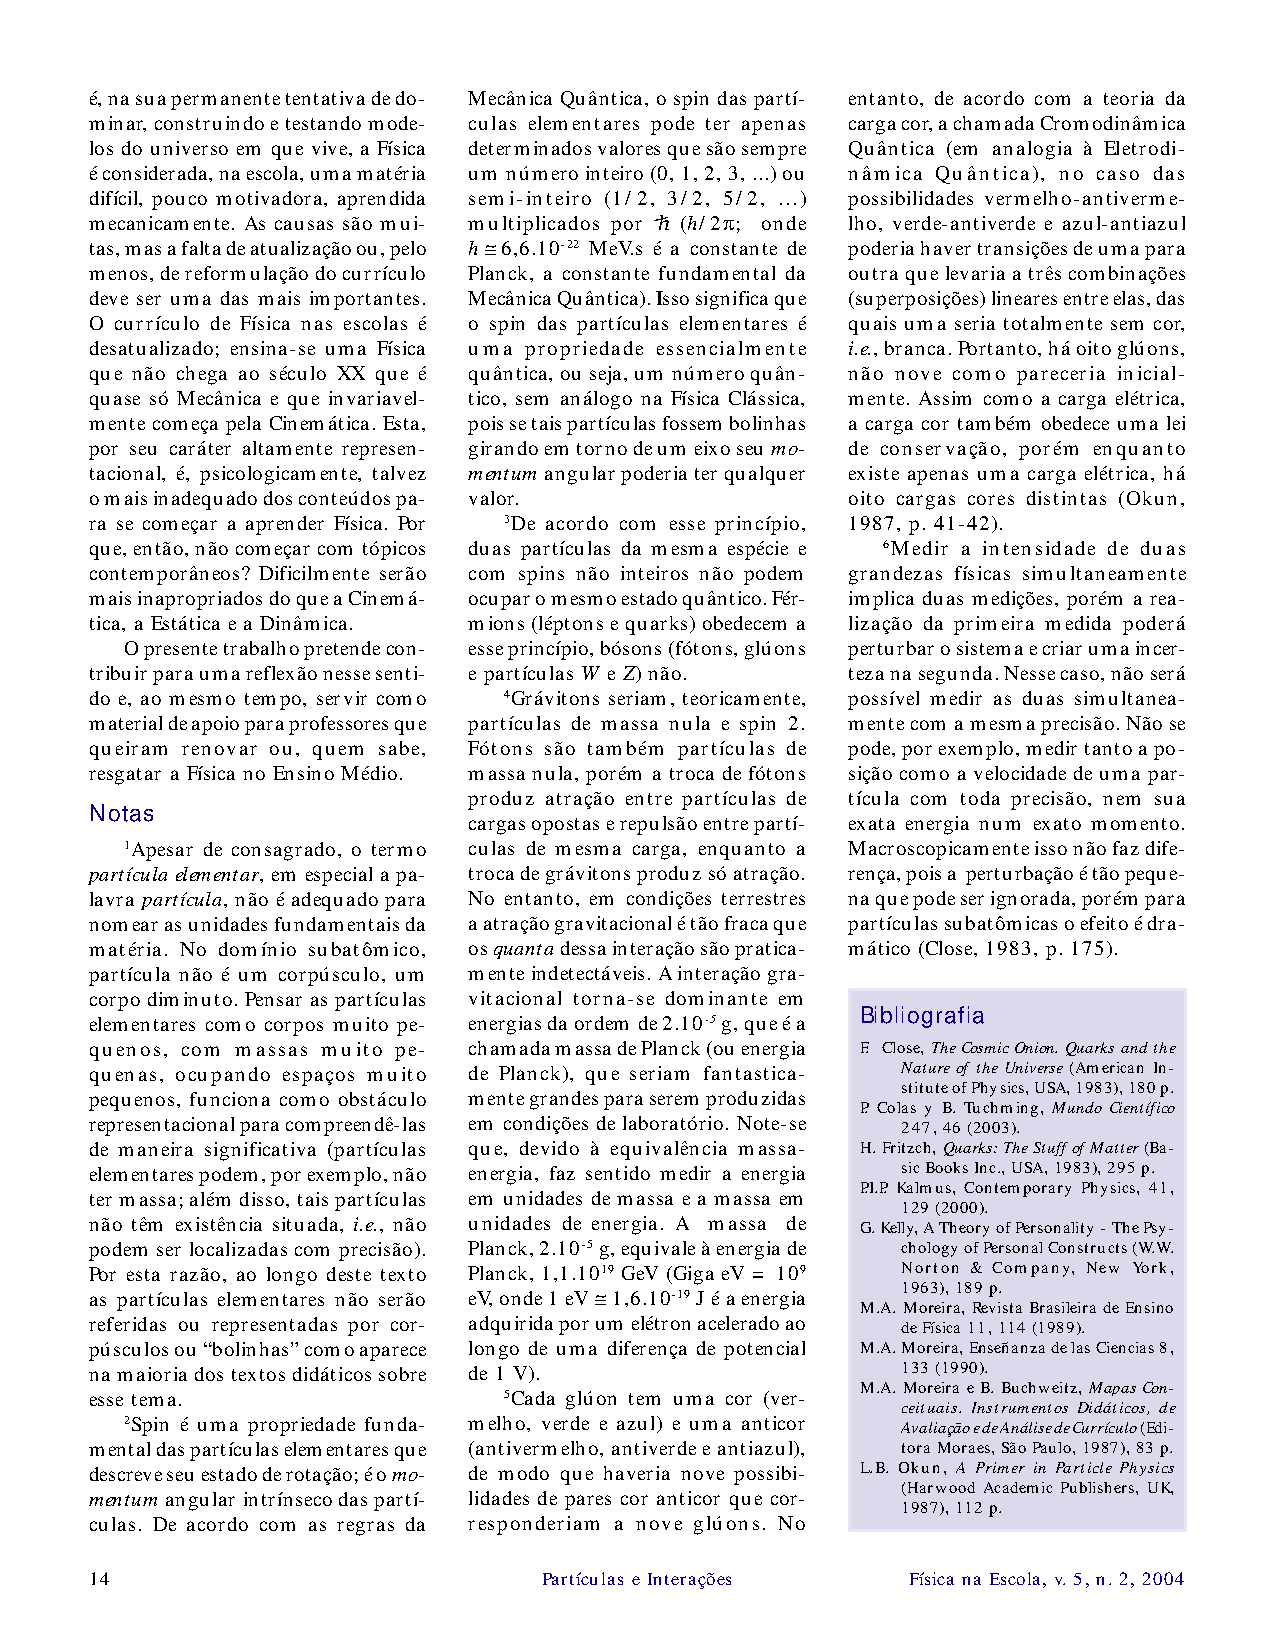
\includegraphics[width=1.0 \textwidth]{AneB/artigo_parte_5}
	\caption{Artigo: Part�culas e Intera��es - P�gina 5}
	\label{fig:artigo_parte_5}
\end{figure}

\section{V�deo}




